\documentclass[12pt,twoside]{article}

\usepackage{amsmath}
\usepackage{color}
\usepackage{enumitem}
\usepackage{graphicx}
\usepackage{booktabs}
\graphicspath{ {images/} }
\usepackage{subfig}
\usepackage{placeins}
\usepackage{float}
\usepackage{mdframed}
\usepackage{booktabs}


\newcommand{\head}[1]{\textnormal{\textbf{#1}}}
\renewcommand{\contentsname}{Table of contents}

\newcommand{\cross}[1][1pt]{\ooalign{%
  \rule[1ex]{1ex}{#1}\cr% Horizontal bar
  \hss\rule{#1}{.7em}\hss\cr}}% Vertical bar

% Cross-references for handout numbers.

\newcommand{\name}{}

\usepackage{latexsym}
%\usepackage{bbm}
\usepackage{times,url}
\usepackage{clrscode}

\newcommand{\mitst}[1]{\begin{description}
\item[MIT students:] #1
\end{description}}
\newcommand{\smast}[1]{\begin{description}
\item[SMA students:] #1
\end{description}}

\newcommand{\profs}{Professor Chris Rycroft}
\newcommand{\subj}{AM205}

\newlength{\toppush}
\setlength{\toppush}{2\headheight}
\addtolength{\toppush}{\headsep}

\newcommand{\htitle}[2]{\noindent\vspace*{-\toppush}\newline\parbox{6.5in}
{\textit{Advanced Scientific Computing: Numerical Methods AM205}\hfill\name\newline
Harvard University \hfill #2\newline
\profs\hfill #1 \vspace*{-.5ex}\newline
\mbox{}\hrulefill\mbox{}}\vspace*{1ex}\mbox{}\newline
\begin{center}{\Large\bf #1}\end{center}}

\newcommand{\handout}[2]{\thispagestyle{empty}
 \markboth{#1}{#1}
 \pagestyle{myheadings}\htitle{#1}{#2}}

\newcommand{\htitlewithouttitle}[2]{\noindent\vspace*{-\toppush}\newline\parbox{6.5in}
{\textit{Introduction to Algorithms}\hfill#2\newline
Massachusetts Institute of Technology \hfill 6.006\newline
%Singapore-MIT Alliance \hfill SMA5503\newline
\profs\hfill Handout #1\vspace*{-.5ex}\newline
\mbox{}\hrulefill\mbox{}}\vspace*{1ex}\mbox{}\newline}

\newcommand{\handoutwithouttitle}[2]{\thispagestyle{empty}
 \markboth{Handout \protect\ref{#1}}{Handout \protect\ref{#1}}
 \pagestyle{myheadings}\htitlewithouttitle{\protect\ref{#1}}{#2}}

\newcommand{\exam}[2]{% parameters: exam name, date
 \thispagestyle{empty}
 \markboth{\subj\ #1\hspace{1in}Name\hrulefill\ \ }%
          {\subj\ #1\hspace{1in}Name\hrulefill\ \ }
 \pagestyle{myheadings}\examtitle{#1}{#2}
 \renewcommand{\theproblem}{Problem \arabic{problemnum}}
}
\newcommand{\examsolutions}[3]{% parameters: handout, exam name, date
 \thispagestyle{empty}
 \markboth{Handout \protect\ref{#1}: #2}{Handout \protect\ref{#1}: #2}
% \pagestyle{myheadings}\htitle{\protect\ref{#1}}{#2}{#3}
 \pagestyle{myheadings}\examsolutionstitle{\protect\ref{#1}} {#2}{#3}
 \renewcommand{\theproblem}{Problem \arabic{problemnum}}
}
\newcommand{\examsolutionstitle}[3]{\noindent\vspace*{-\toppush}\newline\parbox{6.5in}
{\textit{Introduction to Algorithms}\hfill#3\newline
Massachusetts Institute of Technology \hfill 6.006\newline
%Singapore-MIT Alliance \hfill SMA5503\newline
\profs\hfill Handout #1\vspace*{-.5ex}\newline
\mbox{}\hrulefill\mbox{}}\vspace*{1ex}\mbox{}\newline
\begin{center}{\Large\bf #2}\end{center}}

\newcommand{\takehomeexam}[2]{% parameters: exam name, date
 \thispagestyle{empty}
 \markboth{\subj\ #1\hfill}{\subj\ #1\hfill}
 \pagestyle{myheadings}\examtitle{#1}{#2}
 \renewcommand{\theproblem}{Problem \arabic{problemnum}}
}

\makeatletter
\newcommand{\exambooklet}[2]{% parameters: exam name, date
 \thispagestyle{empty}
 \markboth{\subj\ #1}{\subj\ #1}
 \pagestyle{myheadings}\examtitle{#1}{#2}
 \renewcommand{\theproblem}{Problem \arabic{problemnum}}
 \renewcommand{\problem}{\newpage
 \item \let\@currentlabel=\theproblem
 \markboth{\subj\ #1, \theproblem}{\subj\ #1, \theproblem}}
}
\makeatother


\newcommand{\examtitle}[2]{\noindent\vspace*{-\toppush}\newline\parbox{6.5in}
{\textit{Advanced Scientific Computing: Numerical Methods}\hfill#2\newline
Harvard University \hfill AM205 Fall 2017\newline
%Singapore-MIT Alliance \hfill SMA5503\newline
\profs\hfill #1\vspace*{-.5ex}\newline
\mbox{}\hrulefill\mbox{}}\vspace*{1ex}\mbox{}\newline
\begin{center}{\Large\bf #1}\end{center}}

\newcommand{\grader}[1]{\hspace{1cm}\textsf{\textbf{#1}}\hspace{1cm}}

\newcommand{\points}[1]{[#1 points]\ }
\newcommand{\parts}[1]
{
  \ifnum#1=1
  (1 part)
  \else
  (#1 parts)
  \fi
  \
}

\newcommand{\bparts}{\begin{problemparts}}
\newcommand{\eparts}{\end{problemparts}}
\newcommand{\ppart}{\problempart}

%\newcommand{\lg} {lg\ }

\setlength{\oddsidemargin}{0pt}
\setlength{\evensidemargin}{0pt}
\setlength{\textwidth}{6.5in}
\setlength{\topmargin}{0in}
\setlength{\textheight}{8.5in}


\newcommand{\Spawn}{{\bf spawn} }
\newcommand{\Sync}{{\bf sync}}

\renewcommand{\cases}[1]{\left\{ \begin{array}{ll}#1\end{array}\right.}
\newcommand{\cif}[1]{\mbox{if $#1$}}
\newcommand{\cwhen}[1]{\mbox{when $#1$}}

\newcounter{problemnum}
\newcommand{\theproblem}{Problem \theproblemsetnum-\arabic{problemnum}}
\newenvironment{problems}{
        \begin{list}{{\bf \theproblem. \hspace*{0.5em}}}
        {\setlength{\leftmargin}{0em}
         \setlength{\rightmargin}{0em}
         \setlength{\labelwidth}{0em}
         \setlength{\labelsep}{0em}
         \usecounter{problemnum}}}{\end{list}}
\makeatletter
\newcommand{\problem}[1][{}]{\item \let\@currentlabel=\theproblem \textbf{#1}}
\makeatother

\newcounter{problempartnum}[problemnum]
\newenvironment{problemparts}{
        \begin{list}{{\bf (\alph{problempartnum})}}
        {\setlength{\leftmargin}{2.5em}
         \setlength{\rightmargin}{2.5em}
         \setlength{\labelsep}{0.5em}}}{\end{list}}
\newcommand{\problempart}{\addtocounter{problempartnum}{1}\item}

\newenvironment{truefalseproblemparts}{
        \begin{list}{{\bf (\alph{problempartnum})\ \ \ T\ \ F\hfil}}
        {\setlength{\leftmargin}{4.5em}
         \setlength{\rightmargin}{2.5em}
         \setlength{\labelsep}{0.5em}
         \setlength{\labelwidth}{4.5em}}}{\end{list}}

\newcounter{exercisenum}
\newcommand{\theexercise}{Exercise \theproblemsetnum-\arabic{exercisenum}}
\newenvironment{exercises}{
        \begin{list}{{\bf \theexercise. \hspace*{0.5em}}}
        {\setlength{\leftmargin}{0em}
         \setlength{\rightmargin}{0em}
         \setlength{\labelwidth}{0em}
         \setlength{\labelsep}{0em}
        \usecounter{exercisenum}}}{\end{list}}
\makeatletter
\newcommand{\exercise}{\item \let\@currentlabel=\theexercise}
\makeatother

\newcounter{exercisepartnum}[exercisenum]
%\newcommand{\problem}[1]{\medskip\mbox{}\newline\noindent{\bf Problem #1.}\hspace*{1em}}
%\newcommand{\exercise}[1]{\medskip\mbox{}\newline\noindent{\bf Exercise #1.}\hspace*{1em}}

\newenvironment{exerciseparts}{
        \begin{list}{{\bf (\alph{exercisepartnum})}}
        {\setlength{\leftmargin}{2.5em}
         \setlength{\rightmargin}{2.5em}
         \setlength{\labelsep}{0.5em}}}{\end{list}}
\newcommand{\exercisepart}{\addtocounter{exercisepartnum}{1}\item}


% Macros to make captions print with small type and 'Figure xx' in bold.
\makeatletter
\def\fnum@figure{{\bf Figure \thefigure}}
\def\fnum@table{{\bf Table \thetable}}
\let\@mycaption\caption
%\long\def\@mycaption#1[#2]#3{\addcontentsline{\csname
%  ext@#1\endcsname}{#1}{\protect\numberline{\csname
%  the#1\endcsname}{\ignorespaces #2}}\par
%  \begingroup
%    \@parboxrestore
%    \small
%    \@makecaption{\csname fnum@#1\endcsname}{\ignorespaces #3}\par
%  \endgroup}
%\def\mycaption{\refstepcounter\@captype \@dblarg{\@mycaption\@captype}}
%\makeatother
\let\mycaption\caption
%\newcommand{\figcaption}[1]{\mycaption[]{#1}}

\newcounter{totalcaptions}
\newcounter{totalart}

\newcommand{\figcaption}[1]{\addtocounter{totalcaptions}{1}\caption[]{#1}}

% \psfigures determines what to do for figures:
%       0 means just leave vertical space
%       1 means put a vertical rule and the figure name
%       2 means insert the PostScript version of the figure
%       3 means put the figure name flush left or right
\newcommand{\psfigures}{0}
\newcommand{\spacefigures}{\renewcommand{\psfigures}{0}}
\newcommand{\rulefigures}{\renewcommand{\psfigures}{1}}
\newcommand{\macfigures}{\renewcommand{\psfigures}{2}}
\newcommand{\namefigures}{\renewcommand{\psfigures}{3}}

\newcommand{\figpart}[1]{{\bf (#1)}\nolinebreak[2]\relax}
\newcommand{\figparts}[2]{{\bf (#1)--(#2)}\nolinebreak[2]\relax}


\macfigures     % STATE

% When calling \figspace, make sure to leave a blank line afterward!!
% \widefigspace is for figures that are more than 28pc wide.
\newlength{\halffigspace} \newlength{\wholefigspace}
\newlength{\figruleheight} \newlength{\figgap}
\newcommand{\setfiglengths}{\ifnum\psfigures=1\setlength{\figruleheight}{\hruleheight}\setlength{\figgap}{1em}\else\setlength{\figruleheight}{0pt}\setlength{\figgap}{0em}\fi}
\newcommand{\figspace}[2]{\ifnum\psfigures=0\leavefigspace{#1}\else%
\setfiglengths%
\setlength{\wholefigspace}{#1}\setlength{\halffigspace}{.5\wholefigspace}%
\rule[-\halffigspace]{\figruleheight}{\wholefigspace}\hspace{\figgap}#2\fi}
\newlength{\widefigspacewidth}
% Make \widefigspace put the figure flush right on the text page.
\newcommand{\widefigspace}[2]{
\ifnum\psfigures=0\leavefigspace{#1}\else%
\setfiglengths%
\setlength{\widefigspacewidth}{28pc}%
\addtolength{\widefigspacewidth}{-\figruleheight}%
\setlength{\wholefigspace}{#1}\setlength{\halffigspace}{.5\wholefigspace}%
\makebox[\widefigspacewidth][r]{#2\hspace{\figgap}}\rule[-\halffigspace]{\figruleheight}{\wholefigspace}\fi}
\newcommand{\leavefigspace}[1]{\setlength{\wholefigspace}{#1}\setlength{\halffigspace}{.5\wholefigspace}\rule[-\halffigspace]{0em}{\wholefigspace}}

% Commands for including figures with macpsfig.
% To use these commands, documentstyle ``macpsfig'' must be specified.
\newlength{\macfigfill}
\makeatother
\newlength{\bbx}
\newlength{\bby}
\newcommand{\macfigure}[5]{\addtocounter{totalart}{1}
\ifnum\psfigures=2%
\setlength{\bbx}{#2}\addtolength{\bbx}{#4}%
\setlength{\bby}{#3}\addtolength{\bby}{#5}%
\begin{flushleft}
\ifdim#4>28pc\setlength{\macfigfill}{#4}\addtolength{\macfigfill}{-28pc}\hspace*{-\macfigfill}\fi%
\mbox{\psfig{figure=./#1.ps,%
bbllx=#2,bblly=#3,bburx=\bbx,bbury=\bby}}
\end{flushleft}%
\else\ifdim#4>28pc\widefigspace{#5}{#1}\else\figspace{#5}{#1}\fi\fi}
\makeatletter

\newlength{\savearraycolsep}
\newcommand{\narrowarray}[1]{\setlength{\savearraycolsep}{\arraycolsep}\setlength{\arraycolsep}{#1\arraycolsep}}
\newcommand{\normalarray}{\setlength{\arraycolsep}{\savearraycolsep}}

\newcommand{\hint}{{\em Hint:\ }}

% Macros from /th/u/clr/mac.tex

\newcommand{\set}[1]{\left\{ #1 \right\}}
\newcommand{\abs}[1]{\left| #1\right|}
\newcommand{\card}[1]{\left| #1\right|}
\newcommand{\floor}[1]{\left\lfloor #1 \right\rfloor}
\newcommand{\ceil}[1]{\left\lceil #1 \right\rceil}
\newcommand{\ang}[1]{\ifmmode{\left\langle #1 \right\rangle}
   \else{$\left\langle${#1}$\right\rangle$}\fi}
        % the \if allows use outside mathmode,
        % but will swallow following space there!
\newcommand{\paren}[1]{\left( #1 \right)}
\newcommand{\bracket}[1]{\left[ #1 \right]}
\newcommand{\prob}[1]{\Pr\left\{ #1 \right\}}
\newcommand{\Var}{\mathop{\rm Var}\nolimits}
\newcommand{\expect}[1]{{\rm E}\left[ #1 \right]}
\newcommand{\expectsq}[1]{{\rm E}^2\left[ #1 \right]}
\newcommand{\variance}[1]{{\rm Var}\left[ #1 \right]}
\renewcommand{\choose}[2]{{{#1}\atopwithdelims(){#2}}}
\def\pmod#1{\allowbreak\mkern12mu({\rm mod}\,\,#1)}
\newcommand{\matx}[2]{\left(\begin{array}{*{#1}{c}}#2\end{array}\right)}
\newcommand{\Adj}{\mathop{\rm Adj}\nolimits}

\newtheorem{theorem}{Theorem}
\newtheorem{lemma}[theorem]{Lemma}
\newtheorem{corollary}[theorem]{Corollary}
\newtheorem{xample}{Example}
\newtheorem{definition}{Definition}
\newenvironment{example}{\begin{xample}\rm}{\end{xample}}
\newcommand{\proof}{\noindent{\em Proof.}\hspace{1em}}
\def\squarebox#1{\hbox to #1{\hfill\vbox to #1{\vfill}}}
\newcommand{\qedbox}{\vbox{\hrule\hbox{\vrule\squarebox{.667em}\vrule}\hrule}}
\newcommand{\qed}{\nopagebreak\mbox{}\hfill\qedbox\smallskip}
\newcommand{\eqnref}[1]{(\protect\ref{#1})}

%%\newcommand{\twodots}{\mathinner{\ldotp\ldotp}}
\newcommand{\transpose}{^{\mbox{\scriptsize \sf T}}}
\newcommand{\amortized}[1]{\widehat{#1}}

\newcommand{\punt}[1]{}

%%% command for putting definitions into boldface
% New style for defined terms, as of 2/23/88, redefined by THC.
\newcommand{\defn}[1]{{\boldmath\textit{\textbf{#1}}}}
\newcommand{\defi}[1]{{\textit{\textbf{#1\/}}}}

\newcommand{\red}{\leq_{\rm P}}
\newcommand{\lang}[1]{%
\ifmmode\mathord{\mathcode`-="702D\rm#1\mathcode`\-="2200}\else{\rm#1}\fi}

%\newcommand{\ckt}[1]{\ifmmode\mathord{\mathcode`-="702D\sc #1\mathcode`\-="2200}\else$\mathord{\mathcode`-="702D\sc #1\mathcode`\-="2200}$\fi}
\newcommand{\ckt}[1]{\ifmmode \sc #1\else$\sc #1$\fi}

%% Margin notes - use \notesfalse to turn off notes.
\setlength{\marginparwidth}{0.6in}
\reversemarginpar
\newif\ifnotes
\notestrue
\newcommand{\longnote}[1]{
  \ifnotes
    {\medskip\noindent Note: \marginpar[\hfill$\Longrightarrow$]
      {$\Longleftarrow$}{#1}\medskip}
  \fi}
\newcommand{\note}[1]{
  \ifnotes
    {\marginpar{\tiny \raggedright{#1}}}
  \fi}


\newcommand{\reals}{\mathbbm{R}}
\newcommand{\integers}{\mathbbm{Z}}
\newcommand{\naturals}{\mathbbm{N}}
\newcommand{\rationals}{\mathbbm{Q}}
\newcommand{\complex}{\mathbbm{C}}

\newcommand{\oldreals}{{\bf R}}
\newcommand{\oldintegers}{{\bf Z}}
\newcommand{\oldnaturals}{{\bf N}}
\newcommand{\oldrationals}{{\bf Q}}
\newcommand{\oldcomplex}{{\bf C}}

\newcommand{\w}{\omega}                 %% for fft chapter

\newenvironment{closeitemize}{\begin{list}
{$\bullet$}
{\setlength{\itemsep}{-0.2\baselineskip}
\setlength{\topsep}{0.2\baselineskip}
\setlength{\parskip}{0pt}}}
{\end{list}}

% These are necessary within a {problems} environment in order to restore
% the default separation between bullets and items.
\newenvironment{normalitemize}{\setlength{\labelsep}{0.5em}\begin{itemize}}
                              {\end{itemize}}
\newenvironment{normalenumerate}{\setlength{\labelsep}{0.5em}\begin{enumerate}}
                                {\end{enumerate}}

%\def\eqref#1{Equation~(\ref{eq:#1})}
%\newcommand{\eqref}[1]{Equation (\ref{eq:#1})}
\newcommand{\eqreftwo}[2]{Equations (\ref{eq:#1}) and~(\ref{eq:#2})}
\newcommand{\ineqref}[1]{Inequality~(\ref{ineq:#1})}
\newcommand{\ineqreftwo}[2]{Inequalities (\ref{ineq:#1}) and~(\ref{ineq:#2})}

\newcommand{\figref}[1]{Figure~\ref{fig:#1}}
\newcommand{\figreftwo}[2]{Figures \ref{fig:#1} and~\ref{fig:#2}}

\newcommand{\liref}[1]{line~\ref{li:#1}}
\newcommand{\Liref}[1]{Line~\ref{li:#1}}
\newcommand{\lirefs}[2]{lines \ref{li:#1}--\ref{li:#2}}
\newcommand{\Lirefs}[2]{Lines \ref{li:#1}--\ref{li:#2}}
\newcommand{\lireftwo}[2]{lines \ref{li:#1} and~\ref{li:#2}}
\newcommand{\lirefthree}[3]{lines \ref{li:#1}, \ref{li:#2}, and~\ref{li:#3}}

\newcommand{\lemlabel}[1]{\label{lem:#1}}
\newcommand{\lemref}[1]{Lemma~\ref{lem:#1}}

\newcommand{\exref}[1]{Exercise~\ref{ex:#1}}

\newcommand{\handref}[1]{Handout~\ref{#1}}

\newcommand{\defref}[1]{Definition~\ref{def:#1}}

% (1997.8.16: Victor Luchangco)
% Modified \hlabel to only get date and to use handouts counter for number.
%   New \handout and \handoutwithouttitle commands in newmac.tex use this.
%   The date is referenced by <label>-date.
%   (Retained old definition as \hlabelold.)
%   Defined \hforcelabel to use an argument instead of the handouts counter.

\newcounter{handouts}
\setcounter{handouts}{0}

\newcommand{\hlabel}[2]{%
\stepcounter{handouts}
{\edef\next{\write\@auxout{\string\newlabel{#1}{{\arabic{handouts}}{0}}}}\next}
\write\@auxout{\string\newlabel{#1-date}{{#2}{0}}}
}

\newcommand{\hforcelabel}[3]{%          Does not step handouts counter.
\write\@auxout{\string\newlabel{#1}{{#2}{0}}}
\write\@auxout{\string\newlabel{#1-date}{{#3}{0}}}}


% less ugly underscore
% --juang, 2008 oct 05
\renewcommand{\_}{\vrule height 0 pt depth 0.4 pt width 0.5 em \,}


\setlength{\oddsidemargin}{0pt}
\setlength{\evensidemargin}{0pt}
\setlength{\textwidth}{6.5in}
\setlength{\topmargin}{0in}
\setlength{\textheight}{8.5in}

\newcommand{\theproblemsetnum}{}
\newcommand{\releasedate}{December 15, 2017}
\newcommand{\duedate}{December 15, 2017}
\newcommand{\tabUnit}{3ex}
\newcommand{\tabT}{\hspace*{\tabUnit}}

\usepackage{listings}
\usepackage{color}
\usepackage{amsmath}


\definecolor{dkgreen}{rgb}{0,0.6,0}
\definecolor{gray}{rgb}{0.5,0.5,0.5}
\definecolor{mauve}{rgb}{0.58,0,0.82}

\lstset{frame=tb,
  language=Python,
  aboveskip=3mm,
  belowskip=3mm,
  showstringspaces=false,
  columns=flexible,
  basicstyle={\small\ttfamily},
  numbers=none,
  numberstyle=\tiny\color{gray},
  keywordstyle=\color{blue},
  commentstyle=\color{dkgreen},
  stringstyle=\color{mauve},
  breaklines=true,
  breakatwhitespace=true,
  tabsize=3
}





\begin{document}
\thispagestyle{empty}
\newcommand{\HRule}{\rule{\linewidth}{0.5mm}} % Defines a new command for the horizontal lines, change thickness here

\begin{center} % Center everything on the page
\vspace{5mm}

\includegraphics[scale=0.5]{logo_gsas}\\[3cm]
\textsc{\Large Data Science II}\\[0.5cm] % Major heading such as course name
\textsc{\large AC109b}\\[2cm] % Minor heading such as course title

\HRule \\[0.4cm]
{ \huge \bfseries Predicting Cryptocurrency Returns}\\[0.4cm] % Title of your document
\HRule \\[2.5cm]


\begin{minipage}{0.4\textwidth}
\begin{flushleft} \large
\emph{Students:}\\
Ali Dastjerdi\\
Angelina Massa\\
Nate Stein\\
Sachin Mathur\\
\end{flushleft}
\end{minipage}
~
\begin{minipage}{0.4\textwidth}
\begin{flushright} \large
\emph{Professors / Advisor:} \\
Pavlos Protopapas \\
Mark Glickman \\
David Wihl \\
\hspace{1mm}\\
\end{flushright}
\end{minipage}\\[2cm]

{\large \today}\\[2cm]
\end{center}



\newpage
\tableofcontents
\newpage
\setlength{\parindent}{0cm}

\section{Introduction}

Cryptocurrencies are arguably the most polarizing topic within the financial services and financial technology (``fin-tech") community in the last decade. As of April 5, 2018, the market capitalization (``market cap") of cryptocurrencies was over \$255 billion, a number that easily fluctuates by tens of billions of dollars given the immense volatility associated with cryptocurrencies. Billions of dollars more are being invested in cryptocurrency-related start-ups. As one would expect, the number of market participants looking to profit from the change in prices of cryptocurrencies has grown immensely.

\subsection{Problem Statement and Motivation}

Our goal is to build a machine learning model that will enable us to predict the change in the price of a given cryptocurrency that will be realized tomorrow given what we know today. As cryptocurrencies become increasingly accepted as financial assets by mainstream investors, the results from this project and similar predictive modeling exercises have significant implications for investors and market-makers. To build this predictive model, we will experiment with many different types of data, including the trading volume and price history of cryptocurrencies, the price histories of other financial assets, and market-signal features we will engineer using natural language processing (NLP) techniques on financial markets news.

\subsection{Data}

We focus on the following five cryptocurrencies, which, as of 4/1/2018, were among the top 10 cryptocurrencies in terms of market cap on coinmarketcap.com and have data going back to 2015 or earlier: Bitcoin (btc), Ethereum (eth), Ripple (xrp), Litecoin (ltc), and Stellar (xlm). This enables us to have over 900 data points (using daily rolling returns) in our design matrix and use a time frame from 8/8/2015 (the earliest date all five have data available together) to 3/31/2018. Bitcoin and Litecoin have relatively earlier start dates compared to others, but we wanted to encompass a broader universe of cryptocurrencies than just two. Connecting this back to our problem statement, our goal is to build a model that would enable us to predict the price return of one of these five cryptocurrencies by using information on that cryptocurrency's own price history, as well as that of the other four cryptocurrencies and other features.
\bigbreak
In addition to using information about the price and volume history of cryptocurrencies, we will also experiment with the price returns on other financial assets (such as equity indices, bond prices, foreign exchange prices, gold, volatility indices of exchanges, prices of major commodities, etc.). It is one of our hypotheses that the correlation with more traditional financial assets will become stronger (although regarding the direction, we’re not sure about) over the time period analyzed as cryptocurrencies become more mainstream in the investment community.
\subsubsection{Modeling Time Series}
Before delving into the existing literature around this topic, it will help to provide a quick overview on certain features of the problem that will accelerate the reader's understanding of following sections. First, as is common in nearly all financial time series, we are concerned with predicting price \textit{changes}, not the absolute price levels. Therefore, our feature space will consist of relative \textit{changes} in the price and volume traded for certain assets. Moreover, because we are more interested in the trading perspective rather than investing, most of our feature space will consist of \textit{daily} moving windows, as opposed to weekly or monthly, which we discuss in more detail later. A brief visual may help; the following figure shows what the rough work-flow would be if we were attempting to predict the price change for Bitcoin the following day based on the price changes for Bitcoin, Ethereum and Ripple:

\begin{figure}[H]
	\begin{center}
		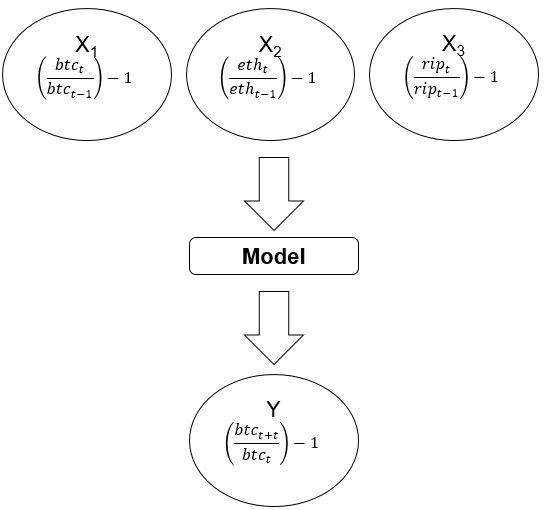
\includegraphics[scale=0.75]{simple_model_graph}
		\caption{Simple Model Illustration}
		\label{fig:simple_model_graph}
	\end{center}
\end{figure}

As described later, the actual feature matrix we use will be significantly more involved. One caveat is that trade-by-trade data may have been more appropriate for attempting to model cryptocurrency price changes from the trading perspective. However, we were unable to find readily available trade-by-trade data for multiple cryptocurrencies, and so we decided to focus on the closest alternative: day-by-day data.

\section{Literature Review}

Unfortunately, there is a dearth of sophisticated analysis on cryptocurrency price return forecasting. Although articles with titles such as ``Use Machine Learning to Predict Bitcoin" abound, they are geared more towards an audience interested in learning software engineering / data science by applying a smattering of techniques to an oversimplified version of the problem. To remedy these inadequacies, we aim to contextualize the problem of cryptocurrency price return forecasting within the broader literature on financial time series analysis.
\bigbreak
Investment approaches are generally bifurcated between (i) ``fundamental" investors, those who value companies based on some estimation of the company's ``true" value based on its assets, profitability, cash flows, etc., and the (ii) ``quantitative" (``quant" for short) investors, who use statistical patterns and machine learning techniques to predict future price changes without regard for the ``true" value of their investments. With cryptocurrencies, no attempt has really been made to estimate their ``true" value, which is not surprising given how relatively new the underlying technology is and to the fact that cryptocurrencies do not lend themselves easily to any sort of parity valuations used with traditional currencies (such as the EUR/USD exchange rate). We focused on ``quant" research for stocks and other traditional financial assets with the aim of drawing parallels to the cryptocurrency focus of this paper. The ultimate hope for these endeavors was that they would inspire ideas for feature engineering and other approaches to our problem. Each of the following subsections centers around summarizing a particular quantitative approach and noting how the existing research influenced how we explored our problem.
\subsection{Momentum}
Momentum is the ``tendency of assets with good (bad) recent performance to continue overperforming (underperforming) in the near future" (Vayanos et al 2013). Han, Yufeng, et al (2013) note that this has been one of the most robust empirical tendencies in financial markets, even though it is, in a way, counterintuitive to those subscribing to the ``buy low, sell high" mentality. The most common ``technical analysis" strategy to profit off this effect is by using a ``moving-average" (MA) strategy whereby an investor buys or continues to hold an investment in an asset when the prior day's price is above its 10-day MA price or invests it into a risk-free asset (such as the 30-day Treasury bill) otherwise. To allow for this effect to potentially be captured by our model, we chose to engineer features capturing whether a given cryptocurrency is above its $x$-day moving price, where we experimented with several different $x$-values, i.e., moving-average windows.
\subsection{Trading Volume}
Vayanos et al (2013) attribute the cause of the momentum effect to some ``shock" (e.g., a news event) that impacts the fundamental value of some assets. For example, in February 2018 a Forbes story broke out that major banks, including J.P. Morgan Chase, Bank of America, and Citigroup would no longer allow their customers to purchase cryptocurrencies using their credit cards. This news could be considered a negative shock to the supposed utility of cryptocurrencies as transactional devices and stores of value. Vayanos et al (2013) argue that the momentum effect occurs as a result of the \textit{gradual} outflows that proceed such a news event, preceded by the large sell-off by major investors. Brown et al (2009) further suggest that trading volume could indeed be a proxy for a number of other important factors, such as liquidity, momentum, and other information. They find that ``past trading volume predicts both the magnitude and the persistence of price momentum." Therefore, trading volume data for cryptocurrencies may enable us to capture momentum and other effects.
\subsection{Covariance between Cryptocurrencies}
Any trading strategy relying on historical price patterns of multiple assets should be especially concerned with conducting a nuanced analysis of the covariance between those assets. This is potentially the most lacking area in existing literature on cryptocurrency price returns. Yan et al (2017) explore the covariance between cryptocurrencies from a variety of different angles and conclude that the covariance between cryptocurrencies, although high, is particularly unstable. This relative instability is true whether we use a basket of stocks from the same sector (such as a basket of energy stocks) or a basket of large-capitalization (large-cap) stocks as our point of reference. This is important for our problem in many ways. First, any incorporation of covariance (even if implicit by virtue of including multiple cryptocurrencies in the design matrix) should permit rolling windows to adjust in some form to ``learn" any changing comovement patterns. Second, this instability will make it difficult to capture any serial dependence in cryptocurrency returns. DeMiguel et al (2014) use vector autoregressive models to select between equity portfolios and find that the expected returns are greater when the principal components can be used to determine which stocks will experience a positive (negative) return in the future. At its least promising, the work done by Yan et al (2017) suggests this would not be possible with cryptocurrencies, while at the most promising, urges caution when basing a model on any assumption of stable comovement.
\bigbreak
The underlying belief in many variants of the autoregressive models is that a given asset occasionally must ``catch up" to other similar assets. As an example commonly given for a traditional attempt at arbitrage, suppose the stock price of PepsiCo, Inc. (ticker: PEP) rises significantly today for no readily identifiable reason, i.e., no news or other announcement was released that would provide new information on the health of PEP as a company. If a very similar stock, such as The Coca-Cola Co (ticker: KO), saw no significant rise in its price today, the argument goes that KO's price will catch up the following day, or, rather potentially, in today's high-speed-trading environment, within hours or seconds.
\bigbreak
This summarizes the description of where we drew inspiration for some of the kinds of features we engineered. The following section will review how we went out about framing our modeling problem and what our process was in determining which features to maintain, tweak, or remove entirely.

\section{Modeling Approach}

Our general approach to modeling mirrors the ``Machine Learning Development Framework," which is illustrated in the following graphic borrowed from a presentation titled ``A Framework for Applying Machine Learning to Systematic Trading":

\begin{figure}[H]
	\begin{center}
		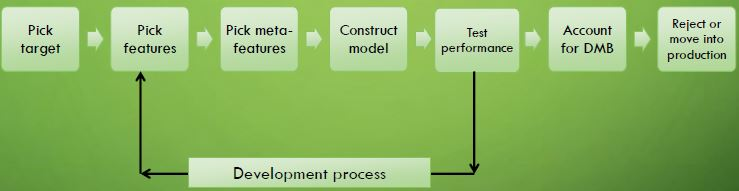
\includegraphics[scale=1.0]{ml_framework_longmore}
		\caption{Machine Learning Framework, taken from Kris Longmore of Quantify Partners}
		\label{fig:ml_framework_longmore}
	\end{center}
\end{figure}

Therefore, the organization of this section will largely mirror the above framework.

\subsection{Selecting Target}

The objective of this project could be addressed in two ways by attempting to predict two related targets:
\begin{enumerate}
	\item The \textit{actual} price return of a given cryptocurrency, which is a regression problem.
	\item The \textit{direction} of the price return for a given cryptocurrency, which can be viewed as a classification problem, with outputs corresponding to trading signals: (+1) Buy (-1) Sell (0) Do Nothing.
\end{enumerate}

\subsubsection{Measuring Performance}

The selection of a target also involves the selection of how to measure performance. In the regression problem, the most easily interpretable performance metric is the mean absolute error (MAE), i.e., the average absolute difference between our predicted price return and the actual price return. The more common mean squared error (MSE) metric is less intuitive since we are typically dealing with decimal numbers smaller than one, and consequently whose square is actually a smaller number. In the classification case, we could approach the problem in a number of ways. We'll compare performance across two metrics: (i) the percentage of Buy/Sell signals that are directionally correct and (ii) the average returns of executing on the Buy/Sell signals. One additional decision to make with the classification problem is what threshold to use when labeling our training data a `Buy'/`Sell' as opposed to a `Do Nothing'. Presumably, we would want to avoid trading when the Buy/Sell signal isn't very strong, so we experiment with varying thresholds.

\subsection{Feature Engineering}

This section provides an overview of the feature space we experimented with. The following section will describe our process for choosing which features to keep in our model.

\subsubsection{Rolling Price and Volume Changes}

Given the methodology suggested by the existing literature in systematic trading, we first introduced lagging variables for the price returns of cryptocurrencies. Implicit in the inclusion of these is the belief that future returns are, to some degree, a function of prior returns. First, let us frame a specific problem to make it clearer. Let's say that on March 28, 2018, we wanted to predict the change in the price of Bitcoin that would occur on the following day (March 29, 2018). We further assume that the decision-maker would wait until the end of the day to make a decision and hence would have at their disposal the return experienced by the cryptocurrencies in scope at the end of March 28, 2018. Therefore, we define the trailing (``rolling") returns as:
$$r_t = \frac{\text{price}_t}{\text{price}_{t-1}} - 1$$

where $\text{price}_t$ is the closing price on 3/28 and $\text{price}_{t-1}$ is the closing price on 3/27. As an example, Bitcoin's closing levels on 3/28 and 3/27 were 7954.48 and 7833.04, respectively, so its daily rolling return on 3/28 is equal to:
$$r_t = \frac{7954.48}{7833.04} - 1=1.55\%$$

We created similar lagging features for the volume traded in cryptocurrencies (where volume is defined as the units bought/sold multiplied by the average price at which those units were bought/sold).

\subsubsection{Preprocessing}

When using lagging financial time series as features, one must make a decision on how to standardize them. A 10\% one-day change in the price of Bitcoin, for example, relays different information depending on when that change was observed. In Figure \ref{fig:ma_returns_std_btc}, we see that the standard deviation of daily returns has changed significantly over time. When we compute the standard deviation of daily returns over rolling 30-day windows, i.e., taking the standard deviation of the daily returns in the 30 observations leading up to and including $t$, we see $\sigma$ is significantly greater towards 2018 than it is in 2016.

\begin{figure}[H]
	\begin{center}
		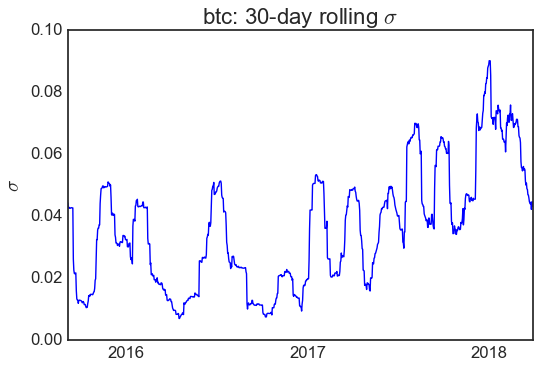
\includegraphics[scale=0.75]{ma_returns_std_btc}
		\caption{$\sigma$ calculated over rolling 30-day periods}
		\label{fig:ma_returns_std_btc}
	\end{center}
\end{figure}

Returning to the original example being addressed, a 10\% one-day change in the price of Bitcoin is more than a 2-$\sigma$ event for most of 2016 while in 2018 it begins to approach being only a 1-$\sigma$ event. Therefore, we decided to standardize each daily rolling return as follows:
$$r^*_t = \frac{r_t - \mu_{t-1}}{\sigma_{t-1}}$$

where 
$$\mu_{t-1}=\frac{1}{30} \sum_{i=t-31}^{t-1} r_i$$

Of course, the number of days to use for this rolling standardization window is, in itself, a meta-feature to our problem.

\subsection{Baseline Model}



\subsection{title}



\section{Conclusion}



\newpage
{\large \textbf{References}}
\bigbreak
Brown, Jeffrey H., et al. ``Trading Volume and Stock Investments." \textit{Financial Analysts Journal}, vol. 65, no. 2, 2009, pp. 67–84.
\bigbreak
Cheng, Evelyn. ``JPMorgan Chase, Bank of America \& Citi bar people from buying bitcoin with a credit card." \textit{cnbc.com}. 2 Feb 2018.
\bigbreak
DeMiguel, Victor, et al. ``Stock Return Serial Dependence and Out-of-Sample Portfolio Performance." \textit{The Review of Financial Studies}, vol. 27, no. 4, 2014, pp. 1031–1073.
\bigbreak
Han, Yufeng, et al. ``A New Anomaly: The Cross-Sectional Profitability of Technical Analysis." \textit{The Journal of Financial and Quantitative Analysis}, vol. 48, no. 5, 2013, pp. 1433–1461.
\bigbreak
Longmore, Kris. ``A Framework for Applying Machine Learning to Systematic Trading." \textit{Quantify Partners}. RobotWealth.com.
\bigbreak
Vayanos, Dimitri, and Paul Woolley. ``An Institutional Theory of Momentum and Reversal." \textit{The Review of Financial Studies}, vol. 26, no. 5, 2013, pp. 1087–1145.
\bigbreak
White, Halbert. ``A Reality Check for Data Snooping." \textit{Econometrica}, vol. 68, no. 5, 2000, pp. 1097–1126.
\bigbreak
Yan, Yihang, et al. ``Do cryptocurrencies move in a parallel manner?." \textit{Harvard University Project}, 2017.
\bigbreak


\end{document}







